\subsection{Kleinste und grösste positive Zahlen}

Es gibt unendlich viele reelle Zahlen. Wir können aber nur endlich viele davon in einem Fliesskommazahlensystem darstellen. Im Kasten, welcher uns die Mantisse veranschaulicht, finden nur endlich viele Bits platz. Das Seil, welches den Kasten an den Komma bindet und welches uns den Exponenten veranschaulicht, hat eine endliche Länge.

Weil es endlich viele darstellbare Zahlen gibt, muss es eine kleinste und eine grösste Zahl geben. In diesem Abschnitt werden wir die kleinste und die grösste positive darstellbare Zahlen finden.


\begin{beispiel}
Wir konstruieren die grösste positive Zahl im Fliesskommazahlensystem mit Mantissenlänge \(5\) und Exponenten von \(-3\) bis \(3\).

In violett wird die reelle Zahl in Basis 2 aufgeschrieben, in der zweiten Zeite kommt die ''Kasten-und-Seil''-Darstellung aus der Einführung, in der dritten Zeite das Bitmuster und als letztes die Exponentialschreibweise. Darstellungsübergreifend ist die Mantisse in braun markiert, der Exponent in Orange und das Vorzeichen in grün.

Als erstes platzieren wir den Kasten. Damit die Zahl möglichst gross wird, muss der Kasten nach links möglichst weit weg vom Komma stehen. Wir haben aber eine Einschränkung: Das Seil muss immer mit dem Komma verbunden bleiben.
\begin{figure}[H]
\centering
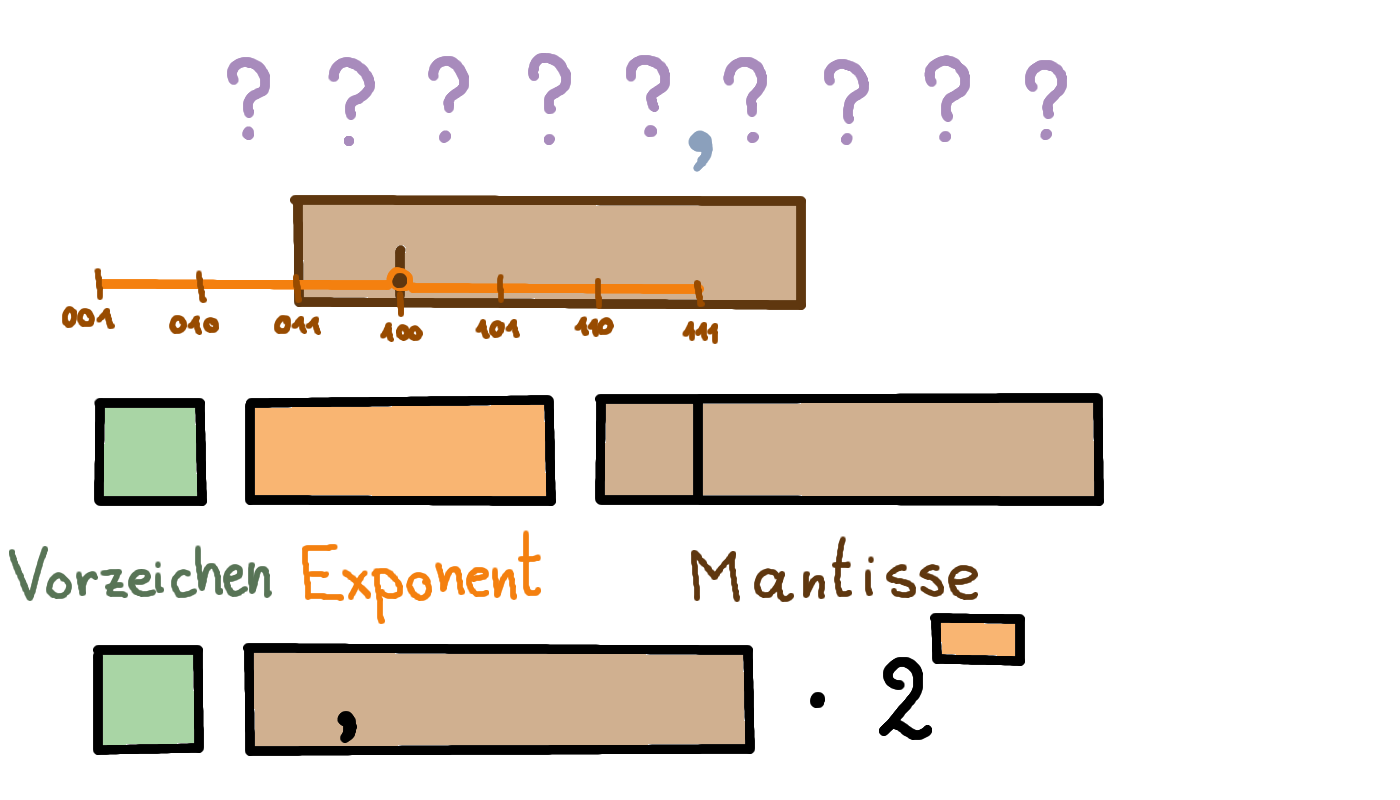
\includegraphics[width=0.85\linewidth]{Pictures/groessteZahl1.png}
\end{figure}
Der Exponent muss also möglichst gross sein.

Was ist mit der Mantisse? Sicher muss eine Eins an der ersten Stelle stehen.
\begin{figure}[H]
\centering
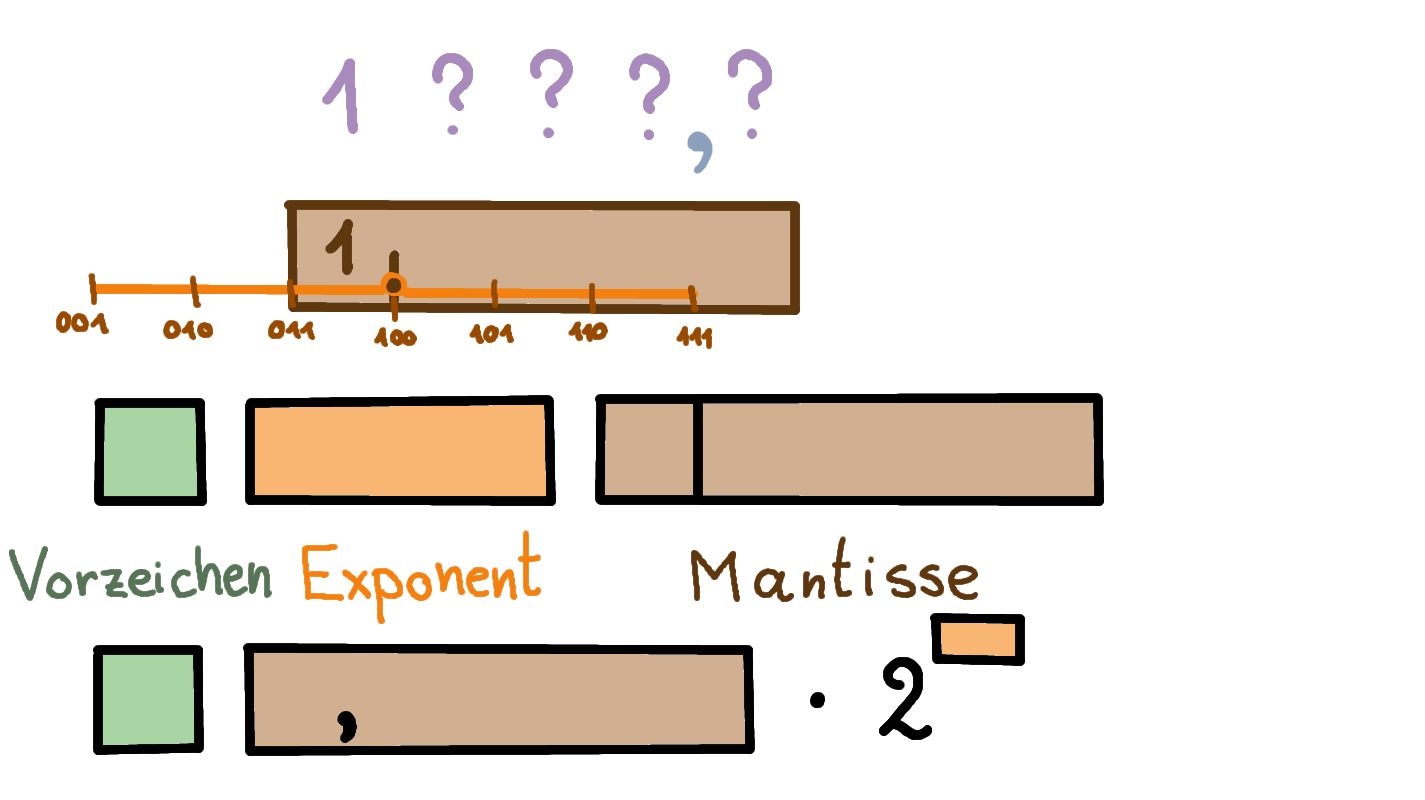
\includegraphics[width=0.85\linewidth]{Pictures/groessteZahl2.png}
\end{figure}

Damit die Mantisse möglichst gross wird, muss sie aus lauter Einser bestehen.
\begin{figure}[H]
\centering
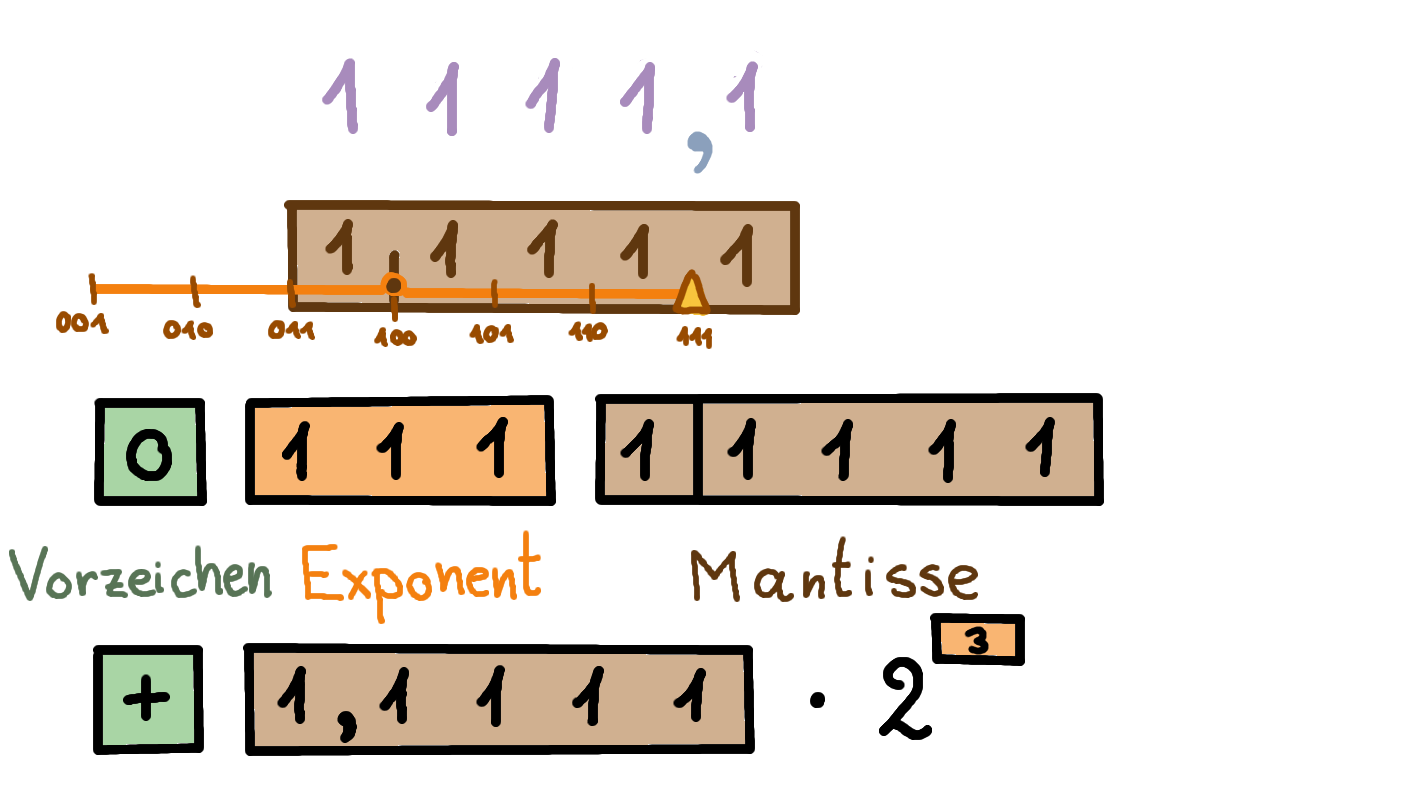
\includegraphics[width=0.85\linewidth]{Pictures/groessteZahl3.png}
\end{figure}

Die grösste darstellbare Zahl in diesem Fliesskommazahlensystem ist also \(15.5\).
\end{beispiel}

\begin{beispiel}
Wir konstruieren die kleinste positive Zahl im Fliesskommazahlensystem mit Mantissenlänge \(5\) und Exponenten von \(-3\) bis \(3\).

Als erstes platzieren wir den Kasten. Damit die Zahl möglichst klein wird, muss der Kasten nach rechts möglichst weit weg vom Komma stehen. Wir haben aber eine Einschränkung: Das Seil muss immer mit dem Komma verbunden bleiben.
\begin{figure}[H]
\centering
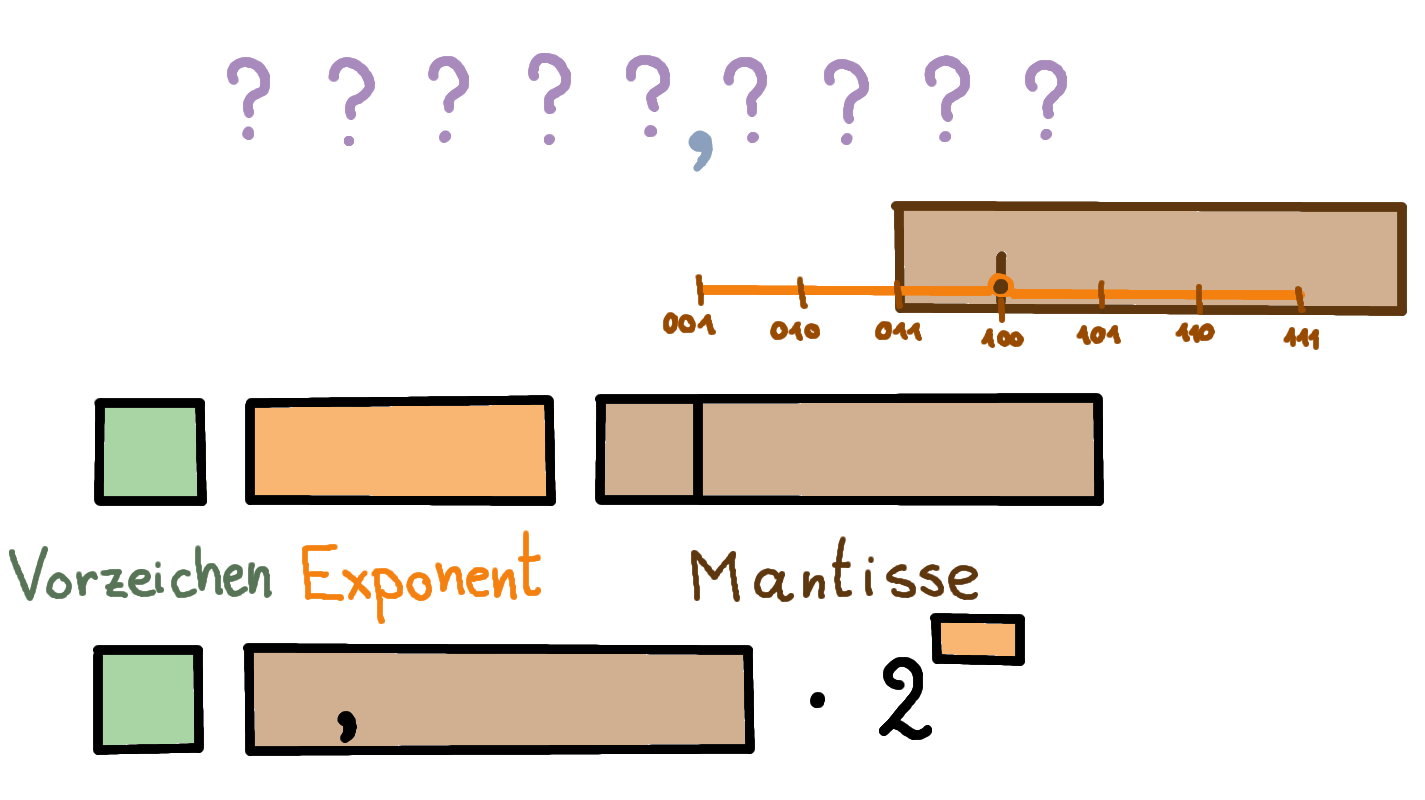
\includegraphics[width=0.85\linewidth]{Pictures/kleinsteZahl1.png}
\end{figure}
Der Exponent muss also möglichst klein sein.

Was ist mit der Mantisse? Sicher muss eine Eins an der ersten Stelle stehen.
\begin{figure}[H]
\centering
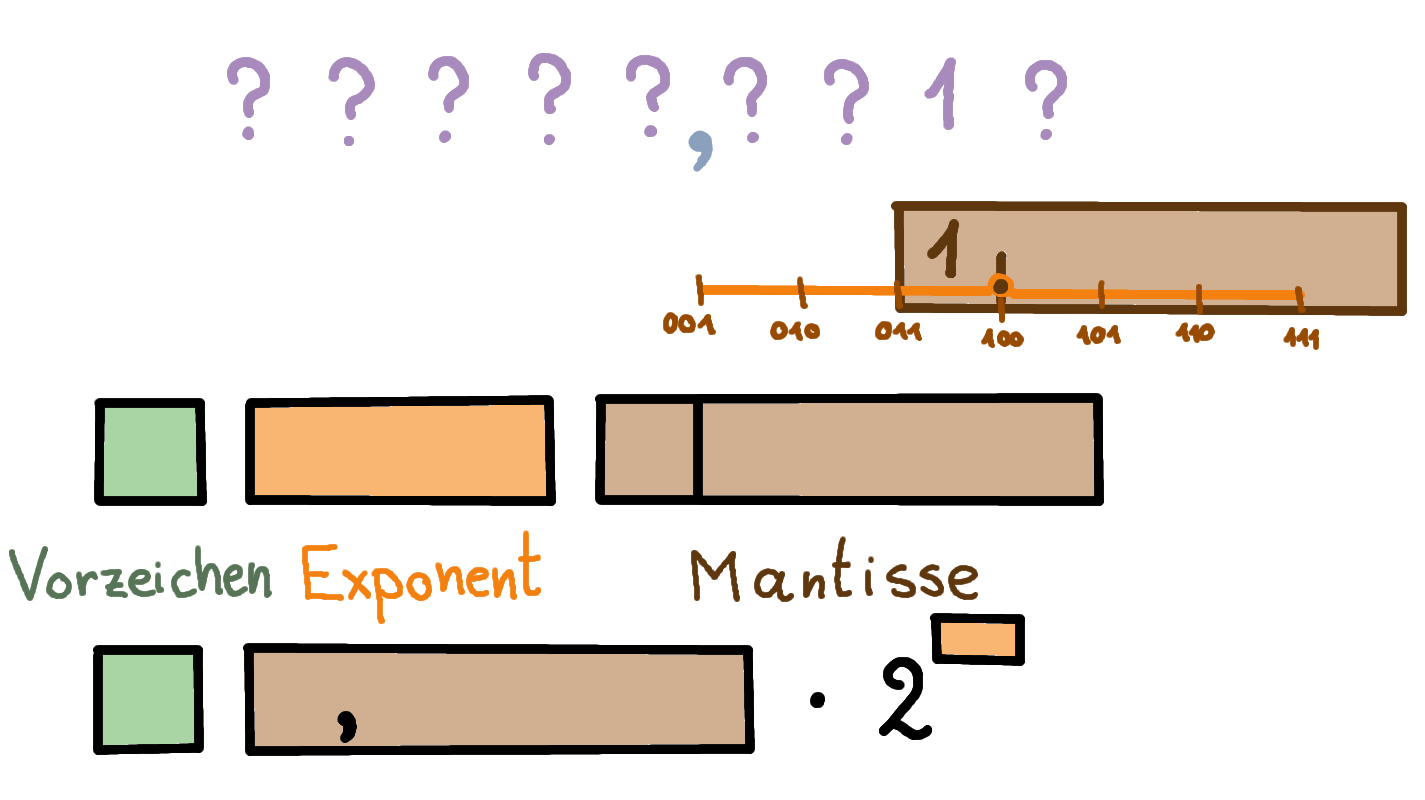
\includegraphics[width=0.85\linewidth]{Pictures/kleinsteZahl2.png}
\end{figure}

Damit die Mantisse möglichst klein wird, müssen wir so viele Stellen wie möglich auf Null setzen.
\begin{figure}[H]
\centering
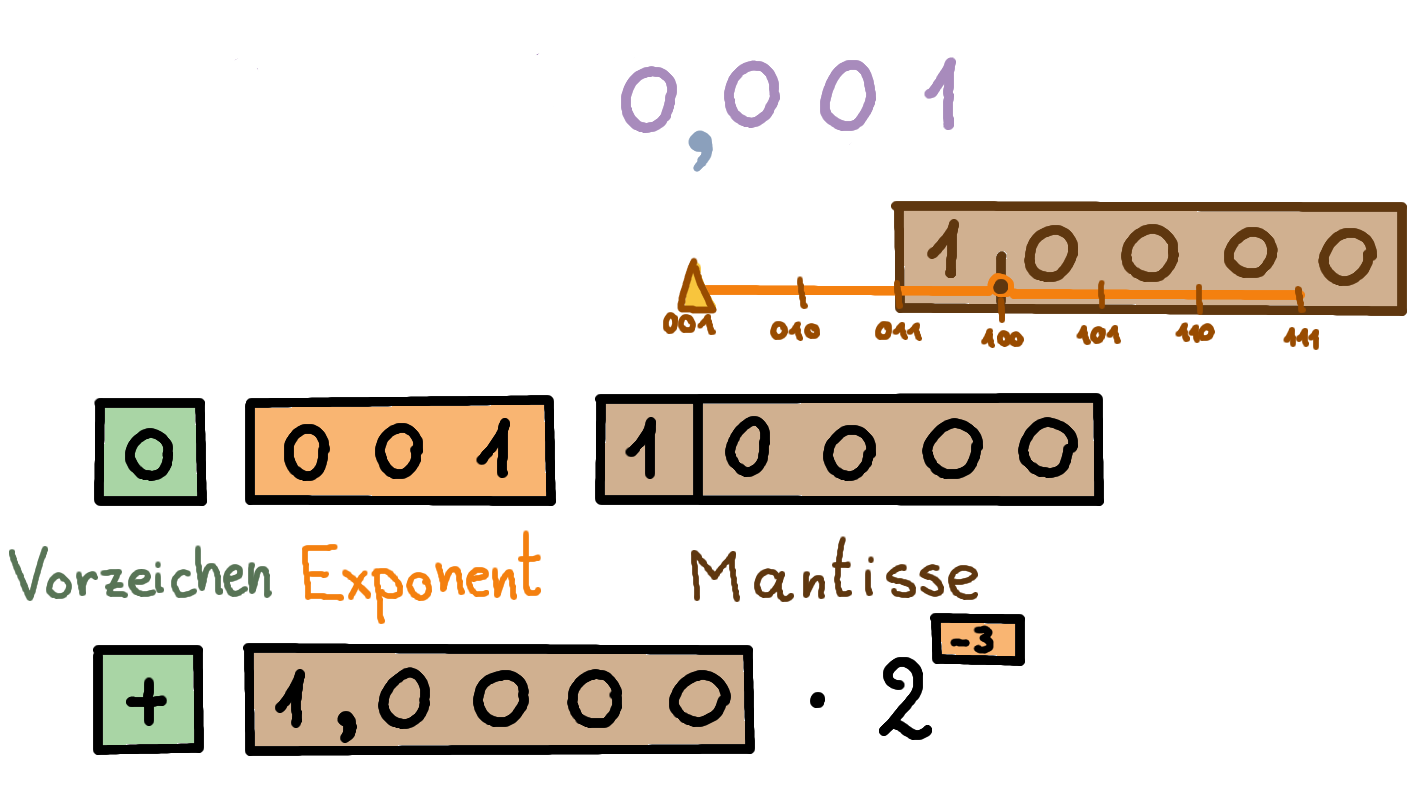
\includegraphics[width=0.85\linewidth]{Pictures/kleinsteZahl3.png}
\end{figure}

Die kleinste darstellbare Zahl in diesem Fliesskommazahlensystem ist also \(1/8\).
\end{beispiel}

\begin{aufgabe}\label{groesste_klein}
Betrachte das Fliesskommazahlensystem mit Mantissenlänge \(3\) und Exponent von \(-1\) bis \(1\). Was sind die grösste und die kleinste darstellbare Zahlen in diesem Fliesskommazahlensystem? Gib den Dezimalwert der Zahl an und stelle sie als Bitmuster und in der Exponentialschreibweise dar.

Für den Exponenten im Bitmuster verwende folgende kodierung: \(01\) kodiert \(-1\), \(10\) kodiert \(0\) und \(11\) kodiert \(1\).
\end{aufgabe}

\begin{aufgabe}
Betrachte das Fliesskommazahlensystem mit Mantissenlänge \(4\) und Exponent von \(-1\) bis \(1\). Was sind die grösste und die kleinste darstellbare Zahlen in diesem Fliesskommazahlensystem? Gib den Dezimalwert der Zahl an und stelle sie als Bitmuster und in der Exponentialschreibweise dar.

Für den Exponenten im Bitmuster verwende folgende kodierung: \(01\) kodiert \(-1\), \(10\) kodiert \(0\) und \(11\) kodiert \(1\).
\end{aufgabe}

Im Allgemeinen für einen Fliesskommazahlensystem mit Mantissenlänge \(m\) und Exponenten zwischen \(e_{min}\) und \(e_{max}\) findet man die grösste und kleinste positive Zahlen wie folgt.

Für die grösste positive Zahl wählt man den grösstmöglichen Exponenten \(e_{max}\) und die grösstmögliche Mantisse \(1.111 \ldots 111\). In der Exponentialschreibweise ist die grösste Zahl also 
\[1.1111111 \ldots 111 \cdot 2^{e_{max}}\]
und hat das Bitmuster \texttt{0 1111...111 (1)111111...111}.

Für die kleinste positive Zahl wählt man den kleinsten möglichen Exponenten \(e_{min}\) und die kleinste mögliche Mantisse. Beachte, dass die Mantisse immer mit einer Eins starten muss. Die kleinste mögliche Mantisse ist deswegen \(1.0000 \ldots 000\). In der Exonentialschreibweise ist die kleinste Zahl also
\[1.0000000 \ldots 000 \cdot 2^{e_{min}}\]
und hat das Bitmuster \texttt{0 0000...001 (1)00000000...000}.


\subsection{Darstellbare Zahlen}

Wir wissen, dass es eine kleinste und eine grösste Zahl gibt. Dass man nicht alle reelle Zahlen zwischen diesen zwei Schranken darstellen kann, können wir uns denken. Die Frage ist nun, welche Zahlen sich darstellen lassen und wie sich der Abstand zwischen darstellbaren Zahlen verhält.

Hier und in den folgenden Kapiteln, falls nicht speziell vermerkt, werden wir mit Mantissenlänge \(5\) und Exponentenbereich von \(-3\) bis \(3\) arbeiten.

\begin{beispiel}
Nehmen wir eine Zahl zwischen 1/8 und 15.5 (die kleinste und grösste darstellbare Zahlen in diesem Fliesskommazahlensystem), zum Beispiel \(10.25\). Lässt sich diese Zahl darstellen?

\begin{figure}[H]
\centering
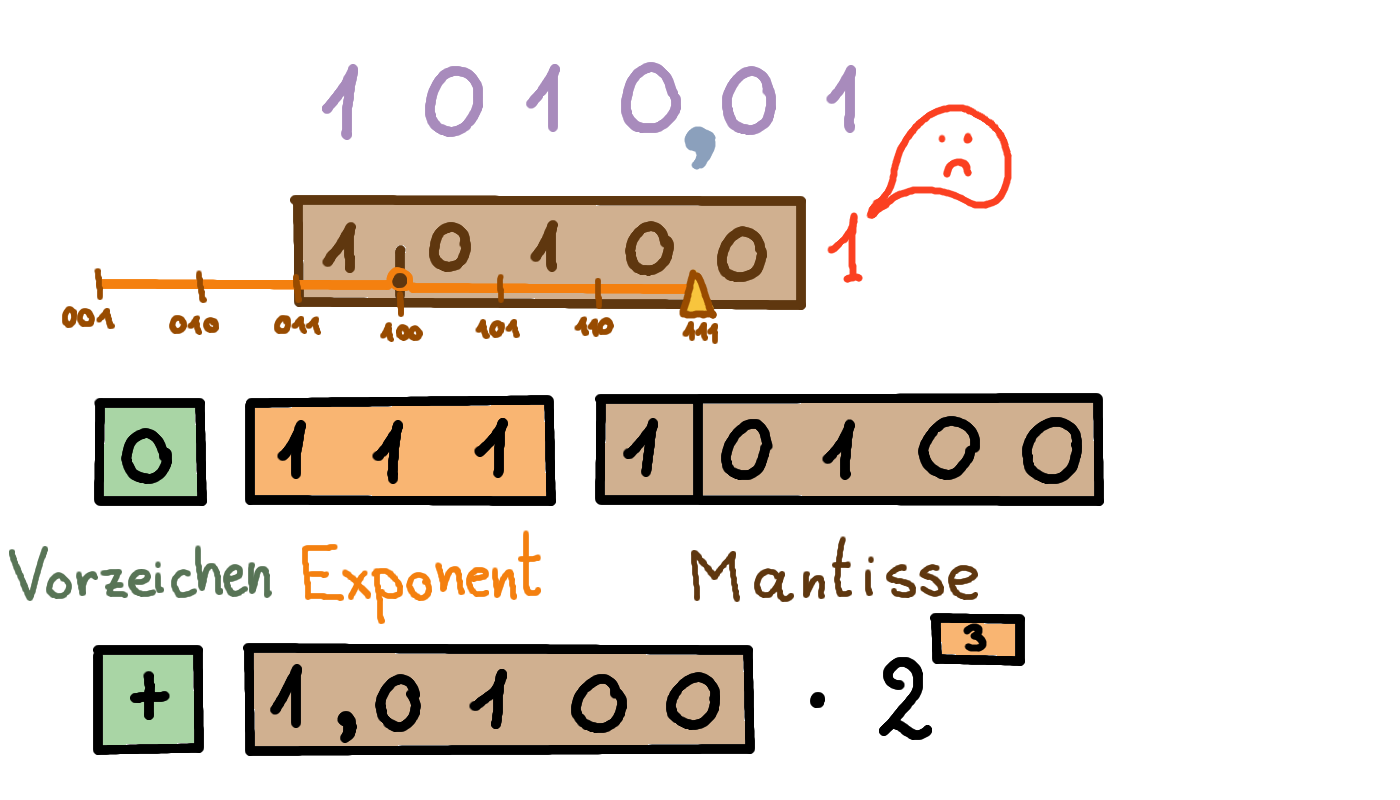
\includegraphics[width=0.75\linewidth]{Pictures/ZahlenDarstellen10-25.png}
\end{figure}

Diese Zahl lässt sich in gegebenem System nicht exakt darstellen. Für die letzte \(1\) gibt es in der Mantisse kein Platz. Deswegen wird \(10.25\) als \(10.0\) dargestellt.
\end{beispiel}

Wir haben gesehen, dass reelle Zahlen sich nur dann exakt darstellen lassen, wenn alle signifikante Stellen in der Mantisse Platz haben.

\begin{beispiel}
Betrachten wir die Zahl \(1\). Was ist die nächstgrösste darstellbare Zahl? Und die nächstkleinste?

Im ersten Schritt werden wir die Zahl \(1\) im gegebenem Fliesskommazahlensystem darstellen.
\begin{figure}[H]
\centering
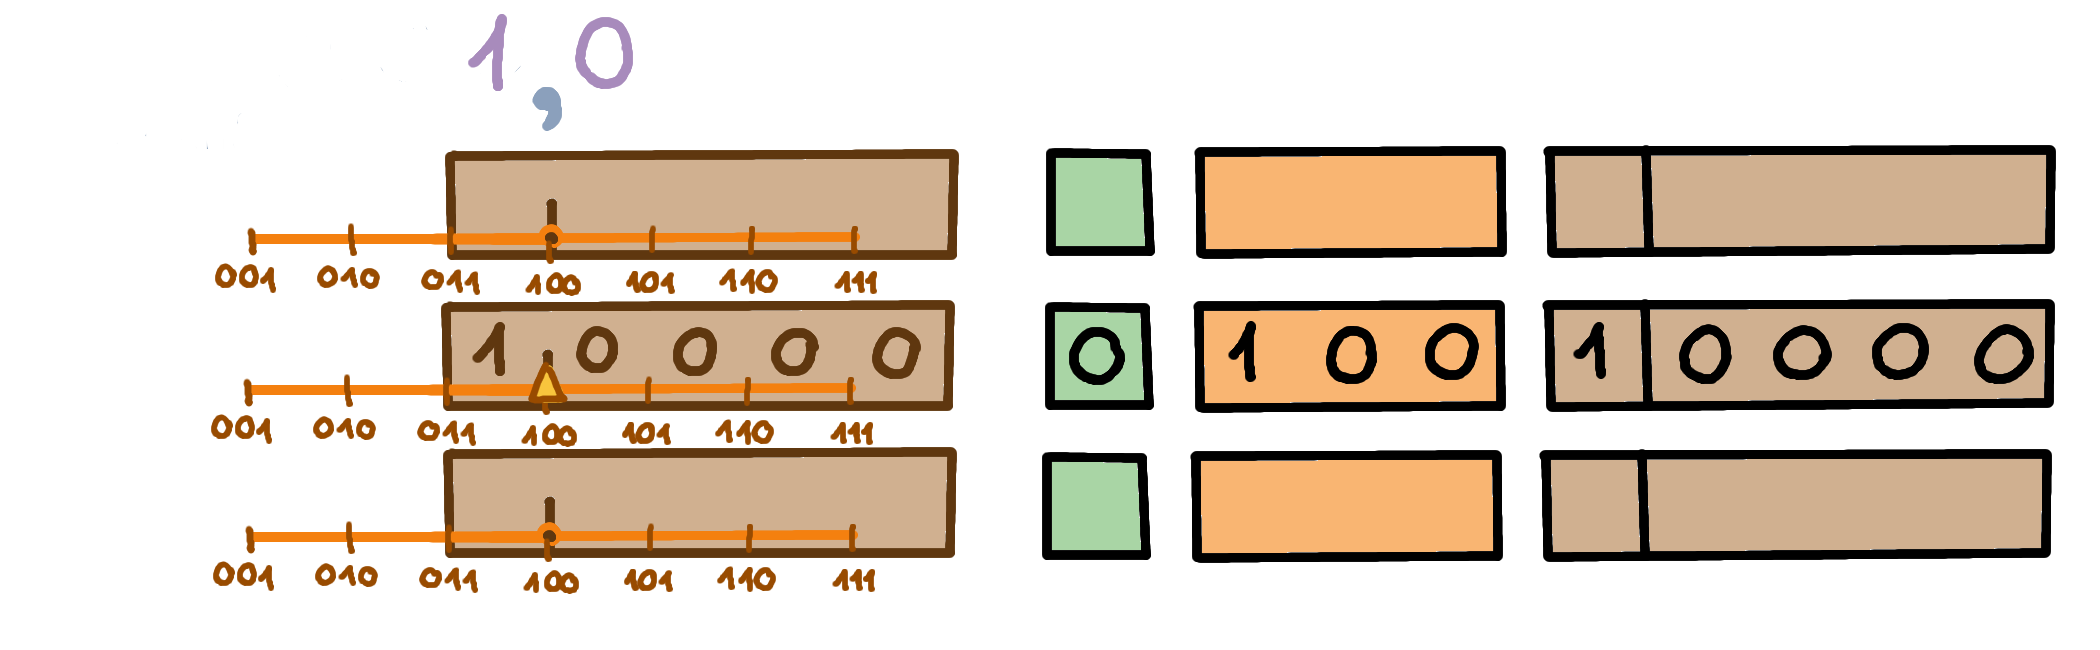
\includegraphics[width=\linewidth]{Pictures/Nachbarn1_1.png} 
\end{figure}

Die nächste darstellbare Zahl finden wir, indem wir in der Mantisse ganz rechts eine Eins addieren.

\begin{figure}[H]
\centering
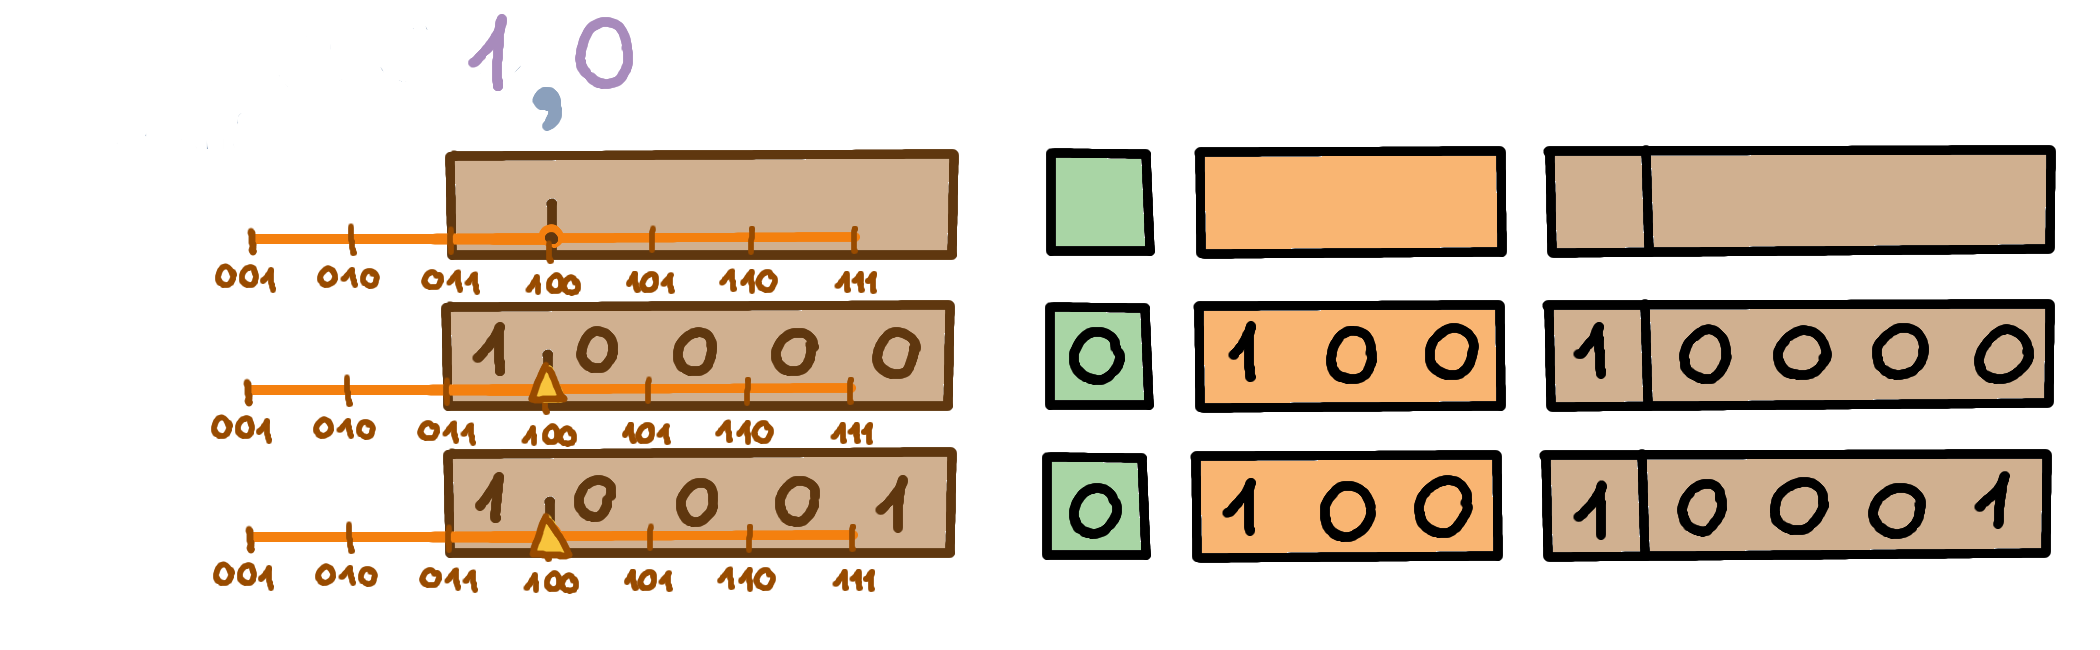
\includegraphics[width=\linewidth]{Pictures/Nachbarn1_N.png} 
\end{figure}
Die nächste darstellbare Zahl ist also \(17/16\).

Die vorherige darstellbare Zahl finden wir, indem wir versuchen die Mantisse kleiner zu machen. Da die Mantisse von \(1\) die kleinste mögliche Mantisse ist, müssen wir den Exponenten um Eins zurücksetzen und die grösstmögliche Mantisse wählen.

\begin{figure}[H]
\centering
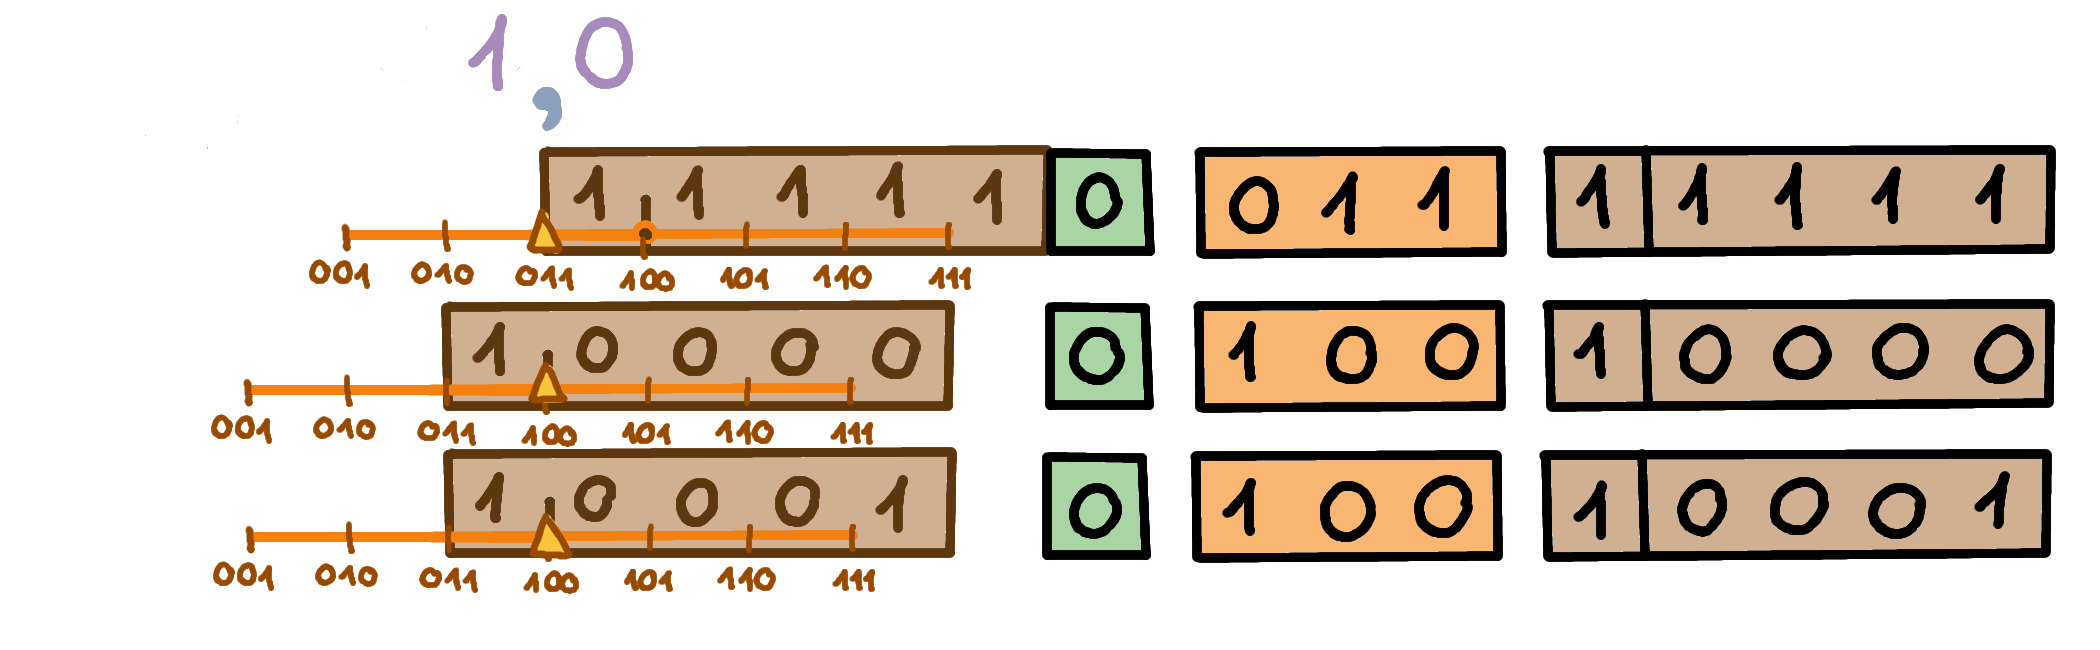
\includegraphics[width=\linewidth]{Pictures/Nachbarn1_P.png} 
\end{figure}
Die vorherige Zahl ist also \(31/32\).

Beachte, dass der Abstand zur nächsten und vorherigen darstellbaren Zahlen in diesem Fall nicht symmetrisch ist: die nächste Zahl ist \(1/16\) entfernt, während die vorherige nur \(1/32\).
\end{beispiel}

\begin{aufgabe}\label{nachbarn}
Finde die nächste und die vorherige darstellbare Zahlen von folgenden Zahlen. Schreibe die Werte in der Dezimaldarstellung auf und stelle alle Zahlen als Bitmuster und in der Exponentialschreibweise dar. Sind alle Nachbarn gleich entfernt?
\begin{enumerate}[(a)]
\item 2
\item 3
\item 4
\end{enumerate}
\end{aufgabe}

\subsubsection*{\textcolor{blue-violet}{Teste dich selber}}

\begin{aufgabe}\label{fliesskommazahlen_kontrollfragen}
Beantworte folgende Fragen:
\begin{enumerate}[(a)]
\item Kann man im Fliesskommazahlensystem alle reelle Zahlen darstellen? Wieso?
\item Gibt es eine grösste Zahl im Fliesskommazahlensystem? Falls nein, warum? Falls ja, wie findet man sie?
\item Gibt es eine kleinste Zahl im Fliesskommazahlensystem? Falls nein, warum? Falls ja, wie findet man sie?
\item Gib eine Zahl zwischen \(1/2\) und \(3.5\) an, die im Fliesskommazahlensystem mit Mantissenlänge 3 und Exponenten von \(-1\) bis \(1\) nicht darstellbar ist.
\item Sind alle Zahlen im Fliesskommazahlensystem gleichverteilt? Falls nicht, welche Zahlen stehen dichter beieinander, die kleineren oder die grösseren?
\end{enumerate}
\end{aufgabe}
